\documentclass[border=3pt]{standalone}
% Preâmbulo compartilhado pelos diagramas TikZ da aula 8 de Navegação (Implementação do RRT)
\usepackage[T1]{fontenc}
\usepackage[utf8]{inputenc}
\usepackage{lmodern}
\usepackage{amsmath}
\usepackage{xcolor}
\usepackage{tikz}
\usetikzlibrary{arrows.meta,angles,quotes,decorations.pathmorphing,decorations.pathreplacing,calc,
                positioning,shapes.geometric,shapes.misc,backgrounds,fit,
                math}

% Paleta (mesma dos SVGs originais)
\definecolor{dblue}{HTML}{2A5B8C}
\definecolor{dorange}{HTML}{B3541E}
\definecolor{dgreen}{HTML}{4A7C59}
\definecolor{dred}{HTML}{9C4B4B}
\definecolor{dcream}{HTML}{F4F1EA}
\definecolor{dshade}{HTML}{DDD7C9}

% Função gaussiana (não normalizada por padrão de escala visual)
\pgfmathdeclarefunction{gauss}{3}{%
  \pgfmathparse{1/(#3*sqrt(2*pi))*exp(-((#1-#2)^2)/(2*#3^2))}%
}

% Estilos comuns (prefixo d... para não colidir com chaves internas do pgf)
\tikzset{
  >={Stealth[length=2mm]},
  dguide/.style={gray!55, dashed, line width=0.4pt},
  daxis/.style={gray!60, line width=0.7pt, ->},
  dbody/.style={fill=black!3, draw=black!80, line width=1pt},
  dacc/.style={draw=dblue, line width=1pt},
  dlbl/.style={black!55, font=\small},
  dsub/.style={black!45, font=\footnotesize},
  dstate/.style={circle, draw=black!80, fill=dcream, line width=1pt,
                 minimum size=17mm, font=\large, inner sep=1pt},
  dobs/.style={circle, draw=black!80, fill=dshade, line width=1pt,
               minimum size=14mm, font=\large, inner sep=1pt},
  dbox/.style={rounded corners=2pt, draw=black!80, fill=dcream, line width=1pt,
               align=center, inner sep=6pt},
  dop/.style={circle, draw=black!80, fill=white, line width=1pt,
              minimum size=6mm, inner sep=0pt, font=\small},
  dtrans/.style={->, dblue, line width=1pt},
  dmeas/.style={->, dorange, line width=1pt},
  dcurve/.style={line width=1pt, dblue},
  dcurveb/.style={line width=1.4pt, dorange},
}

\begin{document}
\hyphenpenalty=10000 \exhyphenpenalty=10000 \tolerance=9999 \emergencystretch=3em
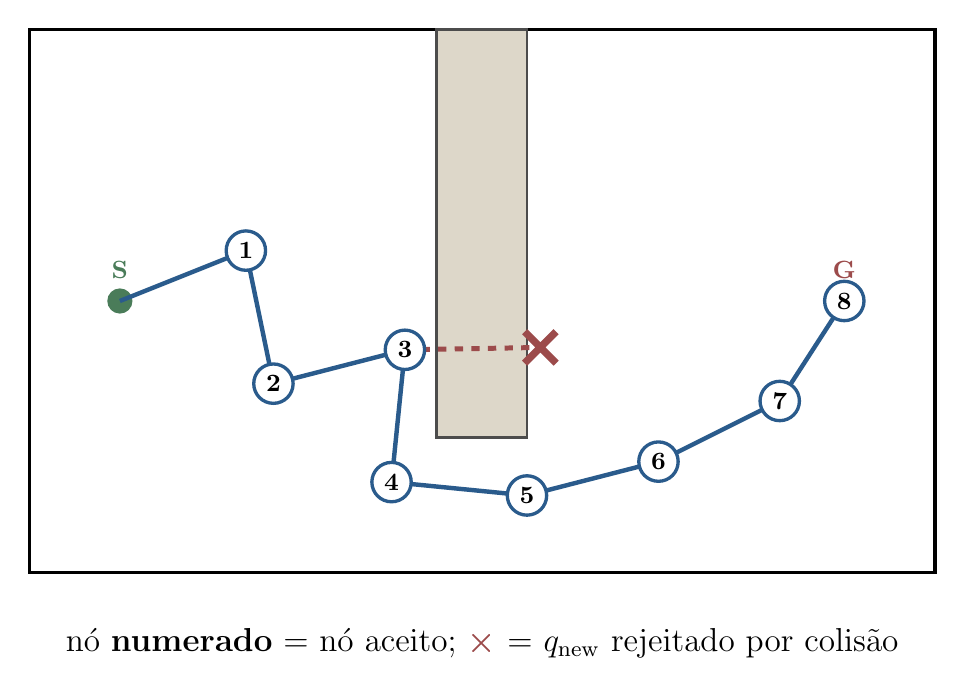
\begin{tikzpicture}[x=1cm,y=1cm]
\draw[line width=1.2pt, fill=white] (0.00,0.00) rectangle (11.50,6.90);
\draw[line width=1pt, draw=black!70, fill=dshade] (5.17,1.72) rectangle (6.32,6.90);
\fill[dgreen] (1.15,3.45) circle (0.16); \node[font=\small\bfseries, text=dgreen, anchor=south] at (1.15,3.61) {S};
\fill[dred] (10.35,3.45) circle (0.16); \node[font=\small\bfseries, text=dred, anchor=south] at (10.35,3.61) {G};
\draw[dblue, line width=1.6pt] (1.15,3.45) -- (2.75,4.09);
\draw[dblue, line width=1.6pt] (2.75,4.09) -- (3.10,2.40);
\draw[dblue, line width=1.6pt] (3.10,2.40) -- (4.77,2.83);
\draw[dred, line width=1.8pt, dashed] (4.77,2.83) -- (6.49,2.86);
\draw[dred, line width=2.6pt] (6.49,2.86) -- ++(0.2,0.2) (6.49,2.86) -- ++(0.2,-0.2) (6.49,2.86) -- ++(-0.2,0.2) (6.49,2.86) -- ++(-0.2,-0.2);
\draw[dblue, line width=1.6pt] (4.77,2.83) -- (4.60,1.15);
\draw[dblue, line width=1.6pt] (4.60,1.15) -- (6.32,0.98);
\draw[dblue, line width=1.6pt] (6.32,0.98) -- (7.99,1.41);
\draw[dblue, line width=1.6pt] (7.99,1.41) -- (9.53,2.18);
\draw[dblue, line width=1.6pt] (9.53,2.18) -- (10.35,3.45);
\node[circle, draw=dblue, fill=white, line width=1.2pt, inner sep=1pt, minimum size=0.5cm, font=\small\bfseries] at (2.75,4.09) {1};
\node[circle, draw=dblue, fill=white, line width=1.2pt, inner sep=1pt, minimum size=0.5cm, font=\small\bfseries] at (3.10,2.40) {2};
\node[circle, draw=dblue, fill=white, line width=1.2pt, inner sep=1pt, minimum size=0.5cm, font=\small\bfseries] at (4.77,2.83) {3};
\node[circle, draw=dblue, fill=white, line width=1.2pt, inner sep=1pt, minimum size=0.5cm, font=\small\bfseries] at (4.60,1.15) {4};
\node[circle, draw=dblue, fill=white, line width=1.2pt, inner sep=1pt, minimum size=0.5cm, font=\small\bfseries] at (6.32,0.98) {5};
\node[circle, draw=dblue, fill=white, line width=1.2pt, inner sep=1pt, minimum size=0.5cm, font=\small\bfseries] at (7.99,1.41) {6};
\node[circle, draw=dblue, fill=white, line width=1.2pt, inner sep=1pt, minimum size=0.5cm, font=\small\bfseries] at (9.53,2.18) {7};
\node[circle, draw=dblue, fill=white, line width=1.2pt, inner sep=1pt, minimum size=0.5cm, font=\small\bfseries] at (10.35,3.45) {8};
\node[font=\large, text width=11cm, align=center] at (5.75,-0.9) {nó \textbf{numerado} = nó aceito; \textcolor{dred}{\textbf{×}} = $q_{\mathrm{new}}$ rejeitado por colisão};
\end{tikzpicture}
\end{document}
